\section{RESULTS}
\label{sec:results}
The results of the proposed experiments are summarized
in \autoref{fig:results} and \autoref{table:results}.
The remaining of this section provides extended descriptions
and interpretation of results.


\begin{table}[h]
\caption{Numerical results}
\label{table:results}
\begin{center}
\begin{tabular}{c||cc|cccc}
\hline
Method & \multicolumn{2}{c|}{Similarity (\%)} & \multicolumn{4}{c}{\gls*{fji} (\%)} \\
\hline
 & B0 & \glspl*{dwi} & Av. & \gls*{csf} & \gls*{wm} & \gls*{gm} \\
\hline
\gls*{fmb} & $80.05$ & $96.26\pm.06$ & $93.00$ & $88.57$ & $96.74$ & $94.02$ \\
\hline
\gls*{reb} & $91.00$ & $97.65\pm.03$ & $96.64$ & $94.31$ & $98.26$ & $96.75$ \\
\hline
\gls*{t2b} & $64.58$ & $90.10\pm.13$ & $79.19$ & $66.31$ & $89.85$ & $82.14$ \\
\hline
\end{tabular}
\end{center}
\end{table}

\begin{figure*}[tpb]
   \centering
   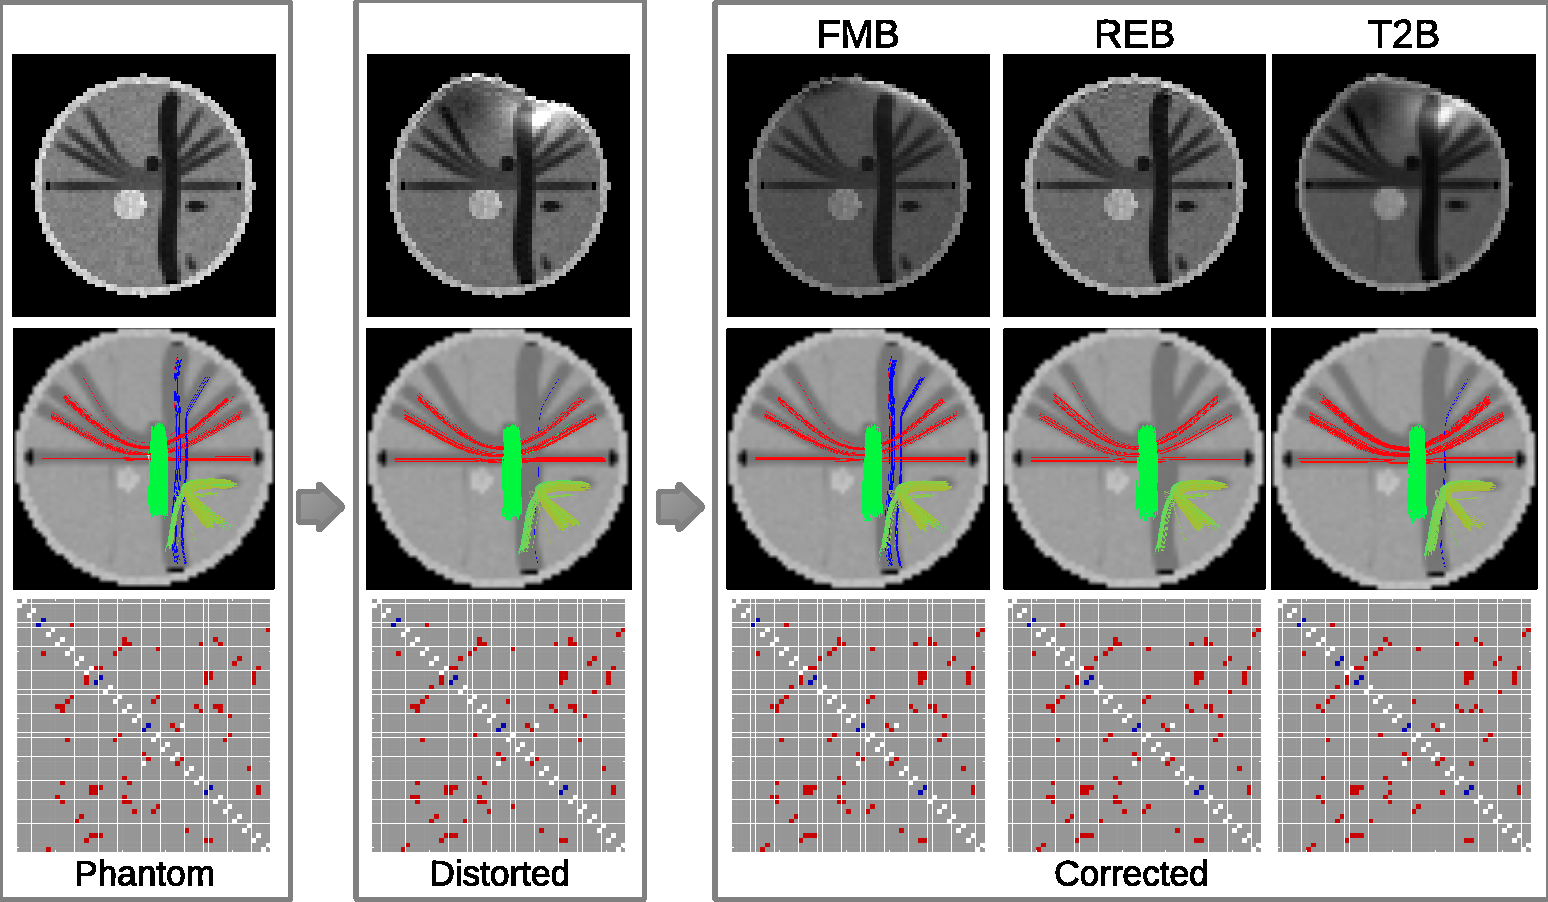
\includegraphics[width=0.9\textwidth]{Fig02-Results}
   \caption{Visual comparison of correction methods results. 
   First row represents
   a coronal section of the \textit{b0} volume. In second row, the outcome
   of tractography, showing only tracks that connect two different
   network nodes. Third row shows the associated connectivity matrix. }
   \label{fig:results}
\end{figure*}


\subsection{Geometrical correctness}

The three methods under study achieved good results in
terms of geometrical accuracy, as it is shown in the first
row of \autoref{fig:results}. The best numerical scores
were obtained with the \gls*{reb} method (\autoref{table:results}),
that achieved a weighted average overlap of $96.64\%$. Second
best were obtained with \gls*{fmb}. Geometrical correctness
is fundamental in connectivity analysis to spatially locate the
\glspl*{roi} that will define the nodes of the final connectivity
matrix. The clear difference of accuracy between \gls*{reb} and \gls*{fmb}
with respect to \gls*{t2b} infers the latter may not be
an appropriate method for susceptibility correction.

\subsection{Signal loss recovery}

A second workflow investigated the similarity of the recovered
signal with respect to the original (undistorted).
In this second study, \gls*{reb} performed significantly
better than the other two methods, as reported
in \autoref{table:results}. \gls*{reb} scored a $91.0\%$
similarity index for the \textit{b0} volume and an average $97.65\%$
for the remaining 31 \glspl*{dwi}. Again, the second
qualified was \gls*{fmb}, which achieved very close results
for the \glspl*{dwi} ($96.26\%$) but not as good for the \textit{b0}
volume. Visual inspection of the recovered data confirms the 
results presented in the Table (\autoref{fig:results}, first
row). Finally, \gls*{t2b} confirmed that its correction
can not be compared, even when using the intensity compensation
based on the determinant of the deformation field.

\subsection{Impact on tractography and connectivity}

The gold-standard contained a total of 1800 valid tracks
connecting regions, with an average length of $40.88\pm8.06$mm.
The corresponding connectivity matrix presented 25 connections 
between the total of 27 different seeding regions.

The distortion of the phantom caused 2 false connections 
(positive connections that are not present on the ground-truth) 
and 2 false negatives (connections vanished).
The correction methods had an adverse impact
on connectivity. Only \gls*{reb} could recover one lost connection
but increasing the false connections count to 3.
\gls*{fmb} ranked second, with 5 false and 2 lost connections.
Finally, \gls*{t2b} presented 9 false and 3 lost connections.

For the sake of completeness, we also document the outcome
of tractography at each step of the workflow. After distortion,
we obtained 1750 tracks and a characteristic length of 
$40.64\pm8.12$mm.
\gls*{fmb} produced 1900 tracks/$40.53\pm8.07$mm., \gls*{reb}
obtained 2200 tracks/$41.15\pm7.60$mm., and 2500 
tracks/$40.60\pm7.81$mm. for \gls*{t2b}. Although track counting has
been used as a measurement of success and as a weight of connectivity 
strength, the number of tracks produced by tractography strongly rely
on the seeding performed and the smoothing caused by interpolation used
within correction methodologies.

\subsection{Discussion}

Even though all the surveyed methods produced visually 
sound results, our study suggested that \gls*{reb} is the 
most accurate methodology for correction of susceptibility-induced
distortions in \gls*{dwi}. Moreover, \gls*{reb} also achieved
the best results in terms of connectivity, being able to recover
one of two lost connections after distortion. \Gls*{fmb} achieved 
very positive scores. Finally, the \gls*{t2b} method did not achieve
the necessary high-standards to recommend its use. We understand
that specific methods with anisotropic regularization that completely
restrict deformations to the phase-encoding direction would perform
significantly better compared to the standard method included
in this study.

One relevant limitation of this work is that the \gls*{fmb} is
used both in distortion creation and correction, what could
bias results. For practical reasons (distortion on the mask, 
signal dropout), the \gls*{fmb} can not achieve a perfect 
geometrical correction as might be
expected if the process was exactly inverse.
Nonetheless, \gls*{reb} performed better that \gls*{fmb}.
A second limitation is found on the impossibility of integrating the
point spread function-based methods for two reasons.
Firstly, the unmet need of a point spread function map consistent
with the synthetic phase-difference map. Secondly, to our knowledge,
there are no implementations of the method readily available.
In practice, this second limitation is narrowed down by the
fact that typical acquisition protocols usually include one or more
datasets among field mapping, reversed-encoding \textit{b0} or T2,
but they do not include the point-spread function mapping.

Future extensions of this work will evaluate
different realizations of the synthetic phase-difference map,
better characterizing the phenomenon. Moreover, the
framework can be enhanced for studying the impact of 
other artifacts as subject's motion or eddy 
currents-derived distortions.